\begin{leftcolumn}
\subsection{Modelo de Costo de Activos de Capital de la empresa (CAPM).}
El fundamento del CAPM establece que los accionistas deben de ganar por su inversión al menos una tasa libre de riesgo, más un diferencial que compense una prima de mercado que contemple el riesgo sistemático de dicha inversión:

\begin{figure}[H]
\centering
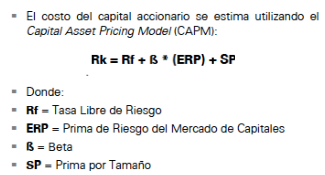
\includegraphics[width=.8\textwidth]{\rutaImagenes/capm}\\
Fuente: Íbid, pag. 46.
\end{figure}

\subsection{Costo de capital (Ke) CAPM 2022.}

Cuanto mayor sea el riesgo sistemático de una acción, más elevado será el rendimiento que los inversionistas esperarán de los títulos accionarios\footnote{William Sharpe.-1934 - a la fecha. Premio Nobel: 1990}.  Dicha estimación utilizó los generadores que se aprecian en la \textcolor{principal}{\textit{Figura 7}}:\\

\begin{figure}[H]
\centering
\includegraphics[width=.8\textwidth]{../0.imagenes/ke}
\end{figure}

Dicha estimación utilizó los generadores y la fórmula que se aprecian en este inciso; con un resultado de: 15.25\% anual (Ke).

\subsubsection}{Costo de la deuda 2022.}

Se recibió por parte del solicitante en el P\&L 2012-2022 información relevante sobre el costo financiero del capital de trabajo involucrado en el negocio  (\textcolor{principal}{\textit{Figura 8}}), a partir del cual se calculó el valor justo de mercado de la deuda antes de impuestos de 15.86\%, cuyo resultado después de aplicar el escudo fiscal es de 11.10\% A/A (KD).\\

\begin{figure}[H]
\centering
\includegraphics[width=\textwidth]{../0.imagenes/kd}
\end{figure}

\subsubsection{Estimación del Costo Promedio Ponderado de Capital.}

 Consiste en la tasa de descuento que debe utilizarse al descontar los flujos de fondos operativos para valuar un intangible. Para determinar una estimación del costo promedio ponderado de capital (WACC) de todo el capital invertido del negocio bajo parámetros de mercado, se utilizó la fórmula que se describe en la \textcolor{principal}{\textit{Figura 9}}; con un resultado de \textbf{WACC= 13.14\% anual}.\\ 

\begin{figure}[H]
\centering
\includegraphics[width=\textwidth]{../0.imagenes/wacc}
\end{figure}

\end{leftcolumn}


\begin{rightcolumn}
\begin{figure}[H]
\centering
\includegraphics[width=\textwidth]{../0.imagenes/ke_1}
\end{figure}

\begin{figure}[H]
\centering
\includegraphics[width=\textwidth]{../0.imagenes/ke_2}
\end{figure}

\begin{figure}[H]
\centering
\includegraphics[width=\textwidth]{../0.imagenes/ke_3}
\end{figure}

\begin{figure}[H]
\centering
\includegraphics[width=\textwidth]{../0.imagenes/ke_4}
\end{figure}

\begin{figure}[H]
\centering
\includegraphics[width=\textwidth]{../0.imagenes/ke_5}
\end{figure}

\begin{figure}[H]
\centering
\includegraphics[width=\textwidth]{../0.imagenes/ke_6}
\end{figure}

\begin{figure}[H]
\centering
\includegraphics[width=\textwidth]{../0.imagenes/ke_7}
\end{figure}

\end{rightcolumn}